
\documentclass{beamer}
\usecolortheme{dove}
\setbeamertemplate{navigation symbols}{}
\usepackage{amsmath,amssymb,amsfonts,amsthm, multicol, subfigure, color}
\usepackage{bm}
\usepackage{graphicx}
\usepackage{tabularx}
\usepackage{booktabs}
\usepackage{hyperref}
\usepackage{pdfpages}
\usepackage{xcolor}
\definecolor{seagreen}{RGB}{46, 139, 87}
\definecolor{ucla}{RGB}{39, 116, 174}
\definecolor{darkestblue}{RGB}{0, 59, 92}
\definecolor{gold}{RGB}{255, 209, 0}
\def\independenT#1#2{\mathrel{\rlap{$#1#2$}\mkern2mu{#1#2}}}
\newcommand\indep{\protect\mathpalette{\protect\independenT}{\perp}}
\def\log{\text{log}}
\newcommand\logit{\text{logit}}
\newcommand\iid{\stackrel{\text{iid}}{\sim}}
\newcommand\E{\text{E}}
\newcommand\V{\text{V}}
\renewcommand\P{\text{P}}
\newcommand{\Cov}{\text{Cov}}
\newcommand{\Cor}{\text{Cor}}
\newcommand\doop{\text{do}}
\usepackage{stackrel}
\usepackage{tikz}
\usetikzlibrary{arrows,shapes.arrows,positioning,shapes,patterns,calc}
\newcommand\slideref[1]{\vskip .1cm \tiny \textcolor{gray}{{#1}}}
\newcommand\red[1]{\color{red}#1}
\newcommand\blue[1]{\color{blue}#1}
\newcommand\gray[1]{\color{gray}#1}
\newcommand\seagreen[1]{\color{seagreen}#1}
\newcommand\purple[1]{\color{purple}#1}
\newcommand\orange[1]{\color{orange}#1}
\newcommand\black[1]{\color{black}#1}
\newcommand\white[1]{\color{white}#1}
\newcommand\teal[1]{\color{teal}#1}
\newcommand\magenta[1]{\color{magenta}#1}
\newcommand\Fuchsia[1]{\color{Fuchsia}#1}
\newcommand\BlueGreen[1]{\color{BlueGreen}#1}
\newcommand\bblue[1]{\textcolor{blue}{\textbf{#1}}}
\newcommand\bred[1]{\textcolor{red}{\textbf{#1}}}
\newcommand\bgray[1]{\textcolor{gray}{\textbf{#1}}}
\newcommand\bgreen[1]{\textcolor{seagreen}{\textbf{#1}}}
\newcommand\bref[2]{\href{#1}{\color{blue}{#2}}}
\colorlet{lightgray}{gray!40}
\pgfdeclarelayer{bg}    % declare background layer for tikz
\pgfsetlayers{bg,main} % order layers for tikz
\newcommand\mycite[1]{\begin{scriptsize}\textcolor{darkgray}{(#1)}\end{scriptsize}}
\newcommand{\tcframe}{\frame{
%\small{
\only<1|handout:0>{\tableofcontents}
\only<2|handout:1>{\tableofcontents[currentsection]}}
%}
}

\usepackage[round]{natbib}
\bibliographystyle{humannat-mod}
\setbeamertemplate{enumerate items}[default]
\usepackage{mathtools}

\newcommand{\goalsframe}{\begin{frame}{Learning goals for today}
At the end of class, you will be able to estimate average causal effects by modeling treatment assignment probabilities. \vskip .2in
Optional reading:
\begin{itemize}
\item Hernán and Robins 2020 Chapter 12.1--12.5, 13, 15.1
\end{itemize}
\end{frame}}

\title{Doubly-Robust Estimation\footnote{Especially today, slides are a high-level overview and we will rely on the website for some technical things.}}
\author{Ian Lundberg\\Soc 212b\\\bref{https://ilundberg.github.io/soc212b}{ilundberg.github.io/soc212b}}
\date{Winter 2025}

\begin{document}

\maketitle

%\goalsframe

\begin{frame}
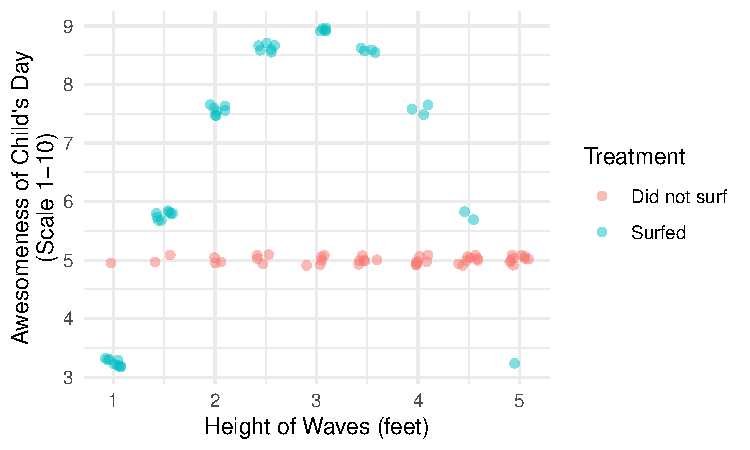
\includegraphics[width = \textwidth]{figures/dr_y.pdf}
\end{frame}

\begin{frame}
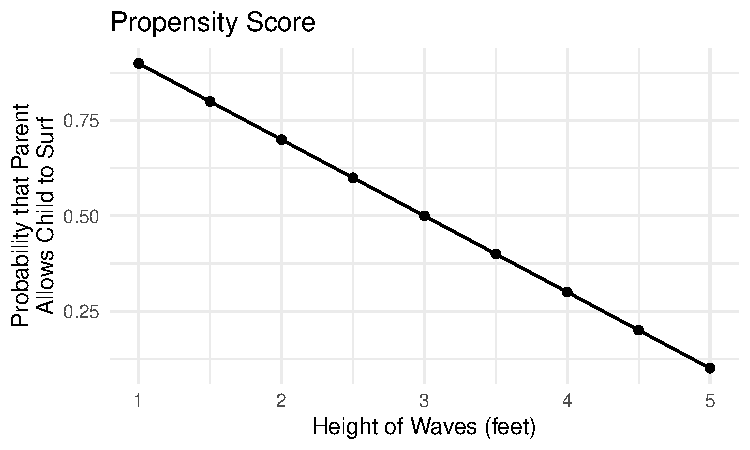
\includegraphics[width = \textwidth]{figures/dr_pscore.pdf}
\end{frame}

\begin{frame}

Child:\\How much more awesome would my day have been if I had surfed on the days when my parents didn't let me?
$$
\text{ATC} = \frac{1}{n_0}\sum_{i:A_i=0} \left(Y_i^1 - Y_i^0\right)
$$

\end{frame}

\begin{frame}

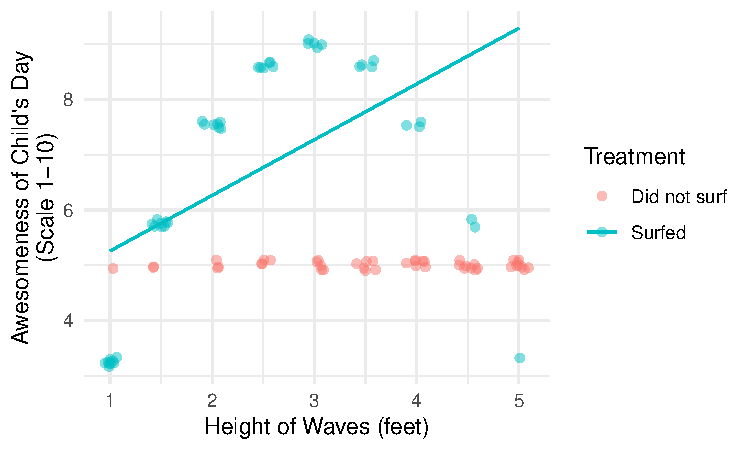
\includegraphics[width = \textwidth]{figures/dr_bestFitLine}

\end{frame}

\begin{frame}

\includegraphics[width = \textwidth]{figures/dr_predictedEffects}

\end{frame}

\begin{frame}

To discuss:
\begin{itemize}
\item In what sense is this line best-fit to the wrong goal?
\item How important is the error at each x-value?
\end{itemize}

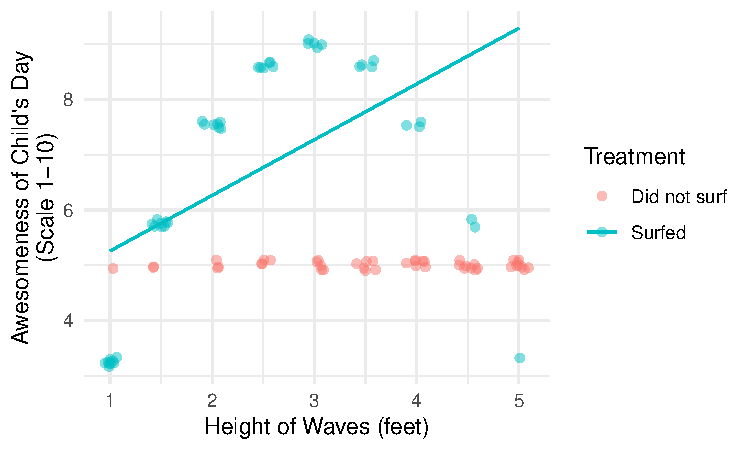
\includegraphics[width = \textwidth]{figures/dr_bestFitLine}

\end{frame}

\begin{frame}

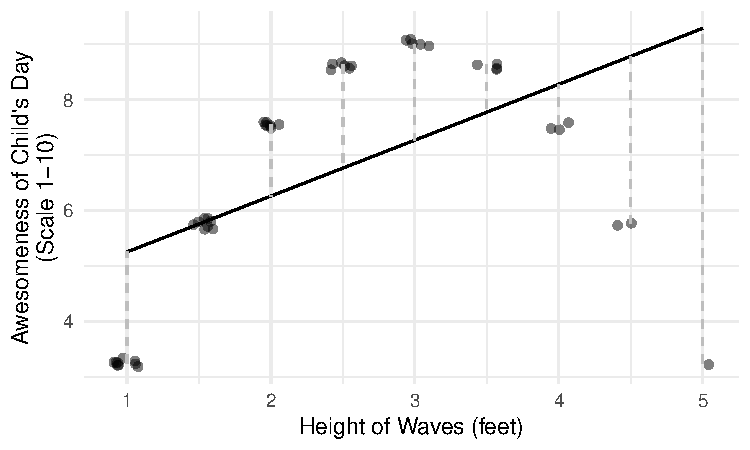
\includegraphics[width = \textwidth]{figures/dr_observedError}

\end{frame}

\begin{frame}

\onslide<2->{Weighted average error: 1.34.}\\
\onslide<3->{Corrected estimate: 2.94 - 1.34 = 1.60}

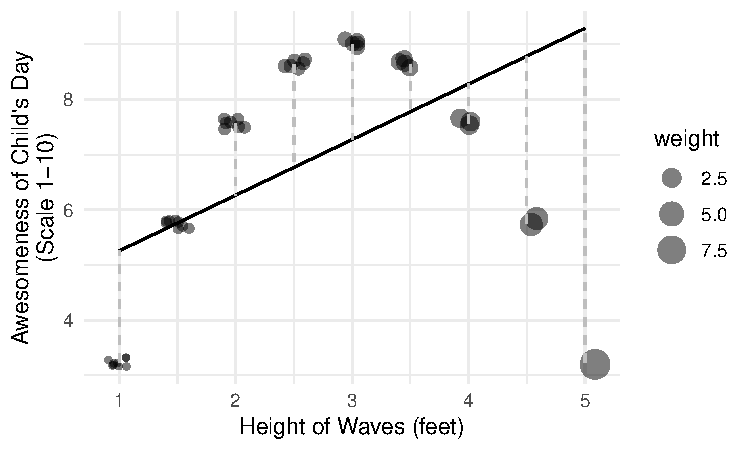
\includegraphics[width = \textwidth]{figures/dr_observedErrorWeighted}

\end{frame}

\begin{frame}{Doubly-robust estimation: Summary}

For the ATC:
\begin{itemize}
\item Predict $\hat{Y}^1$
\item Among treated cases,
\begin{itemize}
\item Weight by $\frac{\hat{P}(A = 1)}{\hat\P(A = 0)}$
\item Take weighted average error: $\hat{Y}^1 - Y$
\item This is a bias correction:\\model was fit at $x$-values of treated cases,\\target to predict is $x$-values of untreated cases
\end{itemize}
\item Among untreated cases, take average $\hat{Y}^1$
\item Then subtract the bias correction
\end{itemize}

\end{frame}


\begin{frame}{Three estimators of $\hat\E(Y^a)$}{What is right when $\hat{g}(a,\vec{x})\rightarrow \E(Y\mid A = a,\vec{X} = \vec{x})$?\\What is right when $\hat{m}(a,\vec{x})\rightarrow \P(A = a\mid \vec{X}  = \vec{x})$?}

$$\begin{aligned}
\hat\tau_\text{Outcome}(a) &= \frac{1}{n}\sum_i \hat{g}(a,\vec{X}_i)\\
\hat\tau_\text{Treatment}(a) &= \frac{1}{\sum_{i:A_i=a}\frac{1}{\hat{m}(A_i,\vec{X}_i)}}\sum_{i:A_i=a} \frac{Y_i}{\hat{m}(A_i,\vec{X}_i)}\\
\hat\tau_\text{AIPW}(a) &= \frac{1}{n}\sum_i \hat{g}(a,\vec{X}_i) \\
	&\qquad -   \frac{1}{\sum_{i:A_i=a}\frac{1}{\hat{m}(A_i,\vec{X}_i)}}\sum_{i:A_i=a} \frac{\hat{g}(A_i,X_i) - Y_i}{\hat{m}(A_i,\vec{X}_i)}
\end{aligned}$$


%with outcome model $\hat{g}(a,\vec{x}) = \hat\E(Y\mid A = a, \vec{X} = \vec{x})$\\
%and treatment model $\hat{m}(a,\vec{x}) = \hat\P(A = a\mid\vec{X} = \vec{x})$

\end{frame}

\begin{frame}{Double robustness: When is each estimator correct?}

With $\hat{g}$ as the outcome model and $\hat{m}$ as the treatment model: \vskip .2in
\begin{tabular}{lccc}
& $\hat\tau_\text{Outcome}(a)$ & $\hat\tau_\text{Treatment}(a)$ & $\hat\tau_\text{AIPW}(a)$ \\
when $\hat{g}$ and $\hat{m}$ are correct & \pause $\checkmark$ & \pause $\checkmark$ & \pause $\checkmark$ \\ \pause
when only $\hat{g}$ is correct & \pause $\checkmark$ & \pause $\times$ & \pause $\checkmark$ \\ \pause
when only $\hat{m}$ is correct & \pause $\times$ & \pause $\checkmark$ & \pause $\checkmark$ \\
\end{tabular}

\end{frame}

\begin{frame}{The problem of overfitting}

Suppose $\hat{g}$ is very complicated
\begin{itemize}
\item e.g. regress $Y$ on $p = 100$ predictors in a sample of $n = 150$
\end{itemize} \vskip .2in
Debiasing relies on errors: $\hat{g}(A,\vec{X}) - Y$
\begin{itemize}
\item What is wrong with these errors?
\item How to fix it?
\end{itemize}

\end{frame}

\begin{frame}{Sample splitting for AIPW}

\begin{enumerate} \pause
\item Split data into sample $\mathcal{S}_1$ and $\mathcal{S}_2$ \\ \pause
\item Using $\mathcal{S}_1$, estimate $\hat{g}$ and $\hat{m}$ \pause
\item Using $\mathcal{S}_2$, calculate the AIPW estimator
\begin{itemize}
\item so that errors are on out-of-sample cases
\end{itemize}
\end{enumerate} \vskip .2in \pause
Popularized as double machine learning (\bref{https://academic.oup.com/ectj/article/21/1/C1/5056401}{Chernozhukov et al. 2018}) \vskip .2in \pause
Concern: Loss of sample size due to splitting. \\ \pause
Answer: Cross fitting. Swap $\mathcal{S}_1$ and $\mathcal{S}_2$. Average result.

\end{frame}

\begin{frame}

\huge Targeted learning

\end{frame}

\begin{frame}{Initial outcome model}

$$
\underbrace{\hat{Q}^0(\vec{x})}_{\substack{\text{The 0 superscript}\\\text{indicates an untargeted}\\\text{initial estimate}}} = \hat{\text{E}}(Y\mid A = 1, \vec{X}) = \hat\alpha + \hat\beta\vec{x}
$$
\centering
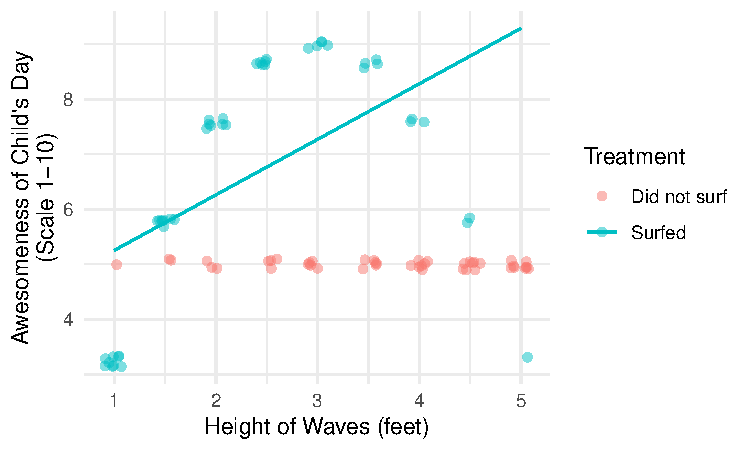
\includegraphics[width = .7\textwidth]{figures/q0}

\end{frame}

\begin{frame}{Clever covariate}

$$
H(x) = \frac{\text{P}(A = \text{Not Surfed} \mid X = x)}{\text{P}(A = \text{Surfed}\mid X = x)}
$$
\centering
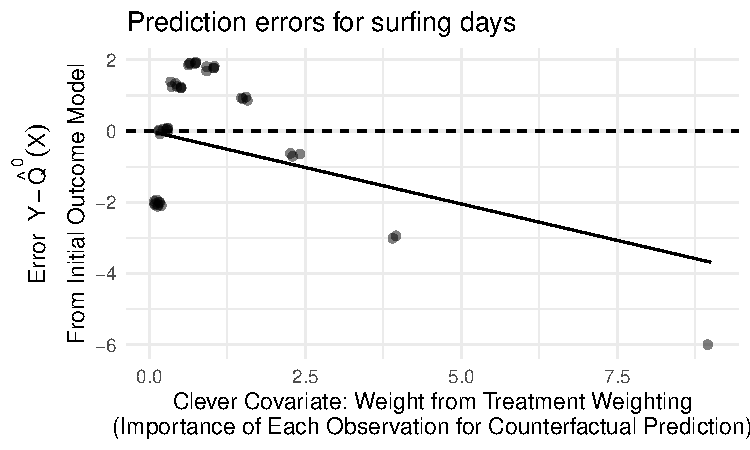
\includegraphics[width = .7\textwidth]{figures/q1}

\end{frame}

\begin{frame}{Targeted outcome model}

$$
\hat{Q}^1(x) = \hat{Q}^0(x) + \hat\gamma \underbrace{\left(\frac{\text{P}(A = \text{Not surfed}\mid X = x)}{\text{P}(A = \text{Surfed}\mid X = x)}\right)}_{\text{Clever covariate }h(x)}
$$
\centering
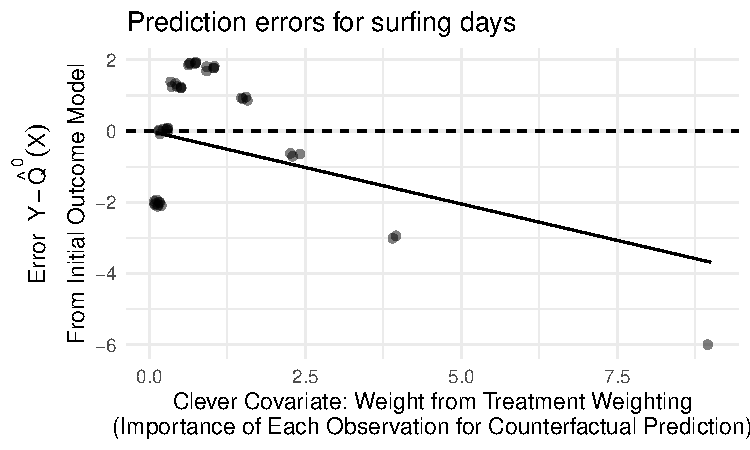
\includegraphics[width = .7\textwidth]{figures/q1}

\end{frame}

\begin{frame}{Initial and targeted estimates}
$$
\begin{aligned}
\text{Estimand:} \qquad && \tau &= \E(Y^\text{Surfed}-Y^\text{Not Surfed}\mid A = \text{Not Surfed}) \\
\text{Initial estimate:}\qquad &&\hat\tau^0 &= \frac{1}{n_{\text{NotSurfed}}}\sum_{i:A_i=\text{NotSurfed}}\left(\hat{Q}^0(x_i) - y_i\right)\\
\text{Targeted estimate:}\qquad &&\hat\tau^1 &= \frac{1}{n_{\text{NotSurfed}}}\sum_{i:A_i=\text{NotSurfed}}\left(\hat{Q}^1(x_i) - y_i\right)
\end{aligned}
$$

\end{frame}

\begin{frame}

Why targeted learning? \pause
\begin{itemize}
\item Doubly robust
\item Intuition: Targeting the outcome model
\item Generalizes to GLM outcome models
\end{itemize}

\end{frame}

\end{document}

\begin{enumerate}
\item Estimate outcome and treatment models
$$
\hat{g}(a,\vec{x}) = \hat\E(Y\mid A = a, \vec{X} = \vec{x})\qquad
\hat{m}(a,\vec{x}) = \hat\P(A = a\mid\vec{X} = \vec{x})
$$
%\begin{itemize}
%\item Outcome model: $\hat{g}(a,\vec{x}) = \hat\E(Y\mid A = a, \vec{X} = \vec{x})$
%\item Treatment model: $\hat{m}(a,\vec{x}) = \hat\P(A = a\mid\vec{X} = \vec{x})$
%\end{itemize}
\item Produce an outcome modeling estimate
$$\hat\tau_\text{Outcome}(a) = \frac{1}{n}\sum_i \hat{g}(a,\vec{X}_i)$$
\item Calculate weighted average error on cases with $A_i = a$
$$
\begin{aligned}
w_i &= \frac{1}{\hat\P(A_i\mid\vec{X}_i)} = \frac{1}{\hat{m}(A_i,\vec{X}_i)} \\
\widehat{\text{Bias}}\left(\hat\tau_\text{Outcome}(a)\right) &= \frac{1}{\sum_{i:A_i=a}w_i}\sum_{i:A_i=a} w_i\left(\hat{g}(a,\vec{X}_i) - Y_i\right)
\end{aligned}
$$
\item De-bias your estimate
$$
\hat\tau_\text{Corrected}(a) = \hat\tau_\text{Outcome}(a) - \widehat{\text{Bias}}\left(\hat\tau_\text{Outcome}(a)\right)
$$
\end{enumerate}

\end{frame}

\begin{frame}{Correction term}

Suppose $\hat{g}(a,\vec{x})\rightarrow \text{E}(Y\mid A = a, \vec{X} = \vec{x})$ for all $\{a,\vec{x}\}$.

To what value does the expected error converge?

$$
\begin{aligned}
&\E\left(\hat{g}(A,\vec{X}) - Y\mid A = a,\vec{X} = \vec{x}\right) \\
&= \E\left(\hat{g}(A,\vec{X})\mid A = a,\vec{X} = \vec{x}\right) - \E\left(Y\mid A = a,\vec{X} = \vec{x}\right) \\
&\rightarrow \E(Y\mid A = a, \vec{X} = \vec{x}) - \E\left(Y\mid A = a,\vec{X} = \vec{x}\right) \\
&= 0
\end{aligned}
$$

%$$
%\begin{aligned}
%&\E\left(\frac{\hat{g}(A,\vec{X}) - Y)}{\hat{m}(A,\vec{X})}\mid A = a\right) \pause \\
%&= 
%\end{aligned}
%$$


%$$
%\frac{1}{\sum_{i:A_i=a} w_i}\sum_{i:A_i=a} w_i\left(\hat{g}(a,\vec{X}_i) - Y_i\right)
%$$

\end{frame}

\begin{frame}{Three estimators}

$$
\begin{aligned}
\text{Outcome modeling} \qquad &  \frac{1}{n}\sum_i \hat{g}(a,\vec{X}_i) \\
\text{Treatment weighting} \qquad & \frac{1}{\sum_{i:A_i=a}w_i}\sum_{i:A_i=a} w_iY_i \\
\text{Augmented IPW} \qquad & \frac{1}{n}\sum_i \hat{g}(a,\vec{X}_i) -{} \\
&\qquad \frac{1}{\sum_{i:A_i=a}w_i}\sum_{i:A_i=a} w_i\left(\hat{g}(A_i,\vec{X}_i) - Y_i\right) \\
\end{aligned}
$$
where $w_i = 1 / \hat{\text{m}}(A_i, \vec{X}_i)$ are inverse probability of treatment weights.

\end{frame}

\goalsframe


\end{document}
